\subsubsectionwithauthor[author={Mika Landeck},email={mika.landeck@fau.de}]{Aufgabe 4: Komplexität}

\paragraph{(a)}m
	Die NP-Härte von $SC$ wird durch eine polynomielle Reduktion auf das bereits als NP-vollständig deklarierte Problem $2VDP$ nachgewiesen. Dazu wird eine totale und berechenbare Funktion $f$ benötigt, die Probleme aus $2VDP$ als kodierte Wörter auf Probleme aus $SC$ abbildet:

	Sei $f:\Sigma^*\rightarrow \Sigma^*$ definiert über

	$f(w)=\begin{cases}
		c(V,E\cup \{(s_2,t_1),(t_2,s_1)\},(s_2,t_1),(t_2,s_1))&, falls\ w=c(V,E,s_1,s_2,t_1,t_2)\\
		&mit\ einem\ Graph\ G=(V,E)\\
		&und\ s_1,s_2,t_1,t_2 \in V\\
		\varepsilon &, sonst
	\end{cases}$

	Die hinter der Konstruktion liegende Idee wird durch folgende Grafik veranschaulicht:

	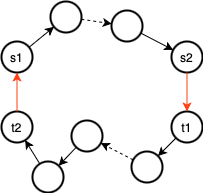
\includegraphics[scale=0.5]{sol/thinf/f23t1/skizze_reduktion.png}
	
	$f$ ist offensichtlich total. Außerdem lässt sich eine DTM konstruieren, die $f$ in polynomieller Laufzeit berechnet:
	\begin{itemize}
		\item Syntaxcheck, ob $w=c(V,E,s_1,s_2,t_1,t_2)$ mit einem Graph $G=(V,E)$ und $s_1,s_2,t_1,t_2 \in V$ (in $O(|V|+|E|)=O(n)$)
		\item Passendes zusammensetzen der Ausgabe zu $c(V,E\cup \{(s_2,t_1),(t_2,s_1)\},(s_2,t_1),(t_2,s_1))$ (in $O(1)$)
	\end{itemize}

	Es bleibt noch zu zeigen, dass $w \in 2VDP \Leftrightarrow f(w) \in SC$ gilt. Dies beweisen folgende Äquivalenzumformungen ($\forall w \in \Sigma^*$):
	\begin{align*}
		w \in 2VDP \Longleftrightarrow\ &w=c(V,E,s_1,s_2,t_1,t_2)\ mit\ Graph\ G=(V,E)\ und\ s_1,s_2,t_1,t_2 \in V\\
		&\wedge\ \exists\ Pfade\ p_1=s_1...s_2\ und\ p_2=t_1...t_2\ in\ G: \forall\ u \in p_1,\ v \in p_2: u\neq v\\
		\Leftrightarrow\ &f(w)=c(V,E\cup \{(s_2,t_1),(t_2,s_1)\}=E',(s_2,t_1),(t_2,s_1))\ mit\ Graph\\
		&\ G'=(V,E')\ und\ s_1,s_2,t_1,t_2 \in V\ \wedge\ \exists\ Pfade\ p_1=s_1...s_2\ und\ p_2=t_1...t_2\ in\ G':\\
		&\ \forall\ u \in p_1,\ v \in p_2: u\neq v\\
		\Leftrightarrow\ &f(w)=c(V,E',(s_2,t_1),(t_2,s_1))\ mit\ Graph\ G'=(V,E')\ und\ (s_2,t_1),(t_2,s_1) \in E'\\
		&\ \wedge\ \exists\ Pfad\ p=s_1...s_2t_1...t_2s_1\ in\ G':\ \forall\ n,m \leq k:=|p| : p_n\neq p_m,\ außer\ p_1=p_k \\
		\Leftrightarrow\ &f(w) \in SC
	\end{align*}
	\textit{Informelle Beschreibung: Zusammensetzen der zwei knoten-disjunkten Pfade über zwei neue Kanten, die jeweils die Endpunkte verbinden, zu einem einfachen Kreis.}

	Somit gilt $2VDP \leq_p SC$ und da $2VDP$ NP-vollständig ist,  muss $SC$ NP-hart sein.
	
	Um noch zu zeigen, dass $SC$ in NP liegt, muss eine NTM skizziert werden, die $SC$ in polynomieller Zeit entscheidet:
	\begin{enumerate}
		\item Starte mit einem leeren Pfad durch den Graphen ($O(1)$).
		\item Rate nun aus den vom letzten Knoten aus erreichbaren Knoten, die noch nicht im Pfad vorkommen (außer dem Startknoten), nichtdeterministisch den nächsten Knoten des Pfades, sodass am Ende (falls dieser existiert) ein Simple Circle gefunden wird ($O(n)$).
		\item Wiederhole den vorherigen Schritt solange, bis der Startknoten wieder erreicht wird - in diesem Fall wurde eine Lösung gefunden $\Rightarrow$ halten und akzeptieren - oder keine weiteren Knoten hinzugefügt werden können - in diesem Fall gibt es keine Lösung $\Rightarrow$ halten und nicht akzeptieren ($O(n)$).
	\end{enumerate}

	Es folgt, dass $SC$ in NP liegt und somit NP-vollständig ist.

\paragraph{(b)}m 
	Folgender Algorithmus löst USC:
	\begin{enumerate}
		\item Überprüfe, ob $e_1 = e_2$.
		\item Falls $e_1 = e_2$ und $e_1=(e_1',e_1''),\ e_2=(e_2',e_2'')$ starte A unter Eingabe $e_1',e_1'',e_2'',e_2'$ \begin{itemize}
			\item Falls A eine Lösung ausgibt, ist der Pfad $p=p_1\circ p_2$ eine Lösung von USC
			\item Falls A keine Lösung findet, gibt es auch für USC keine Lösung
		\end{itemize}
		\item Falls $e_1 \neq  e_2$ und $e_1=(e_1',e_1''),\ e_2=(e_2',e_2'')$ starte A unter Eingabe $e_1'',e_2'',e_2',e_1'$ \begin{itemize}
			\item Falls A eine Lösung ausgibt, ist der Pfad $p=p_1\circ e_2'e_2''\circ p_2\circ e_1'e_1''$ eine Lösung von USC
			\item Falls A keine Lösung findet, gibt es auch für USC keine Lösung
		\end{itemize}
	\end{enumerate}
	\textit{Anmerkung: $\circ $ meint hier die Aneinanderreihung oder Konkatenation von Pfaden. Dabei werden die Knoten in den Pfaden zusammen hintereinander geschrieben, wobei der letzte Knoten des ersten Pfades mit dem ersten Knoten des zweiten Pfades übereinstimmen muss und nur einmal nidergeschrieben wird. Bsp.: $abc\circ cde=abcde,\ \forall a,b,c,d,e \in V$.}

	\textbf{Laufzeitanalyse:}\\
	Die Überprüfung in Schritt 1, das Starten von A sowie die Überprüfung und Rückgabe in Schritt 2 und 3 laufen jeweils in $O(1)$. Der Durchlauf von A in Schritt 2 und 3 hat höchstens eine polynomielle Laufzeit in der Größe der Eingabe, da U2VDP in $\mathcal{P}$ liegt.\\
	Somit hat der beschriebene Algorithus insgesamt höchstens eine polynomielle Laufzeit in der Größe der Eingabe.

	Folglich liegt USC in $\mathcal{P}$.

